\clearpage
\section{Package Diagram}\label{sec:package-diagram}

Il codice di DriveHub è organizzato sotto il package radice \code{it.unifi.ing.drivehub} in quattro parti principali. \code{presentation} gestisce le schermate JavaFX, i controller e la navigazione; \code{business} coordina i casi d'uso e le strategie di calcolo; \code{dao} definisce le interfacce di persistenza e le implementa tramite JDBC; \code{domain} raccoglie le entità e le regole proprie dei veicoli e delle operazioni. Le frecce del diagramma indicano la direzione delle dipendenze: i servizi usano le interfacce DAO, l'implementazione PostgreSQL usa quelle interfacce e le entità, mentre il dominio non dipende dagli altri tre livelli.

\begin{figure}[H]
  \centering
  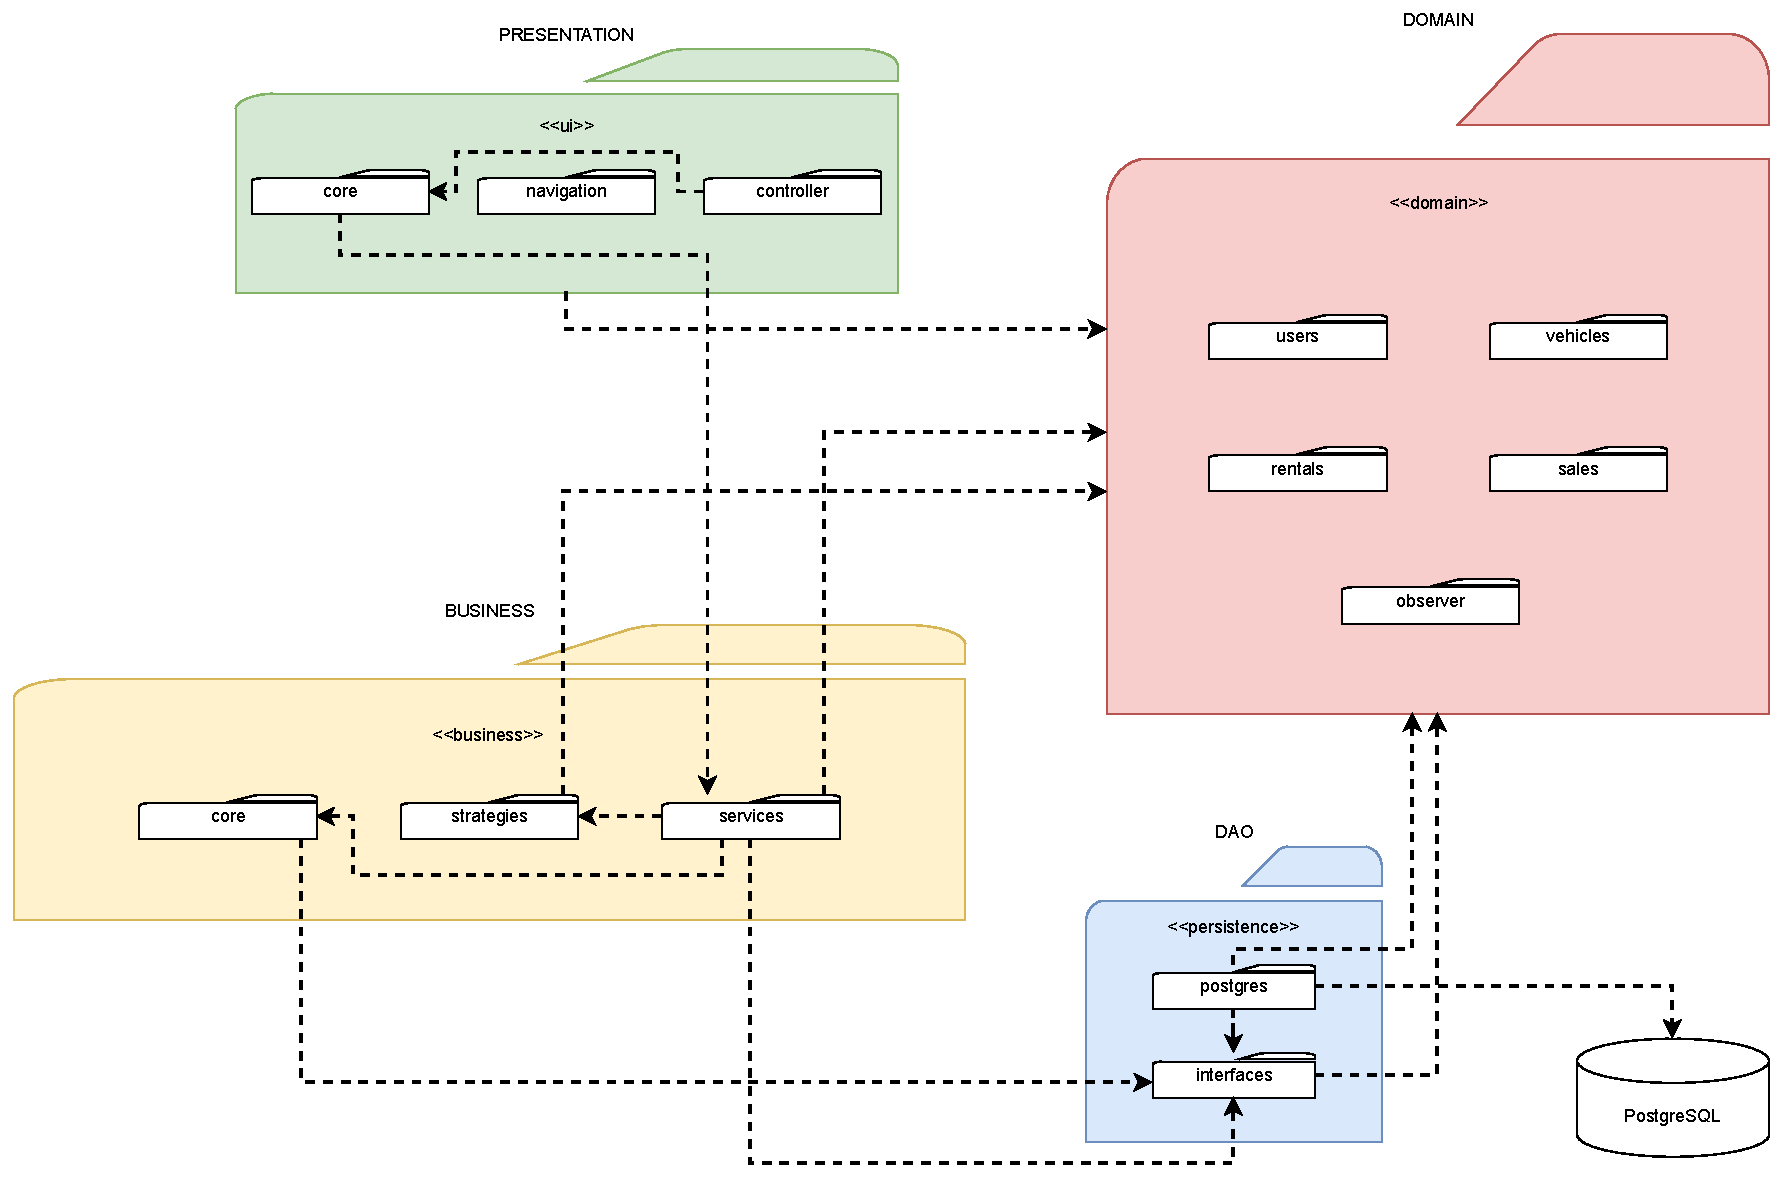
\includegraphics[width=.95\textwidth,height=.68\textheight,keepaspectratio]{package-diagram-original.pdf}
  \caption{Diagramma dei package di DriveHub e delle loro dipendenze.}\label{fig:package-attuale}
\end{figure}

\subsection*{Il dominio non dipende dagli altri livelli}

Le classi del package \code{domain} non importano classi di \code{presentation}, \code{business} o \code{dao}: le entità non conoscono né le schermate né il modo in cui vengono salvate. Nel diagramma le dipendenze entrano nel dominio, senza frecce in uscita verso gli altri livelli. Questa separazione permette di applicare e verificare le regole delle entità indipendentemente dall'interfaccia JavaFX e da PostgreSQL.

La separazione ha un effetto concreto in \code{Vehicle}: i metodi \code{approve}, \code{block} e \code{unblock} controllano lo stato corrente prima di modificarlo, senza affidare questa regola al controller o al DAO. Anche \code{BankAccount} verifica nel dominio che un prelievo non superi il saldo disponibile. I servizi coordinano queste operazioni; le condizioni proprie delle entità restano nelle classi che le rappresentano. Nel disegno le frecce \code{controller} $\rightarrow$ \code{presentation.core} e \code{presentation.core} $\rightarrow$ \code{business.services} rispecchiano il passaggio dai controller a \code{UiGateway} e poi a \code{ServiceUiGateway}, che invoca i servizi.
